\documentclass[border=5mm]{standalone}
\usepackage{tikz}
\usetikzlibrary{patterns.meta, arrows.meta, calc}
\usepackage{amsmath}
\usepackage{amssymb}

\begin{document}

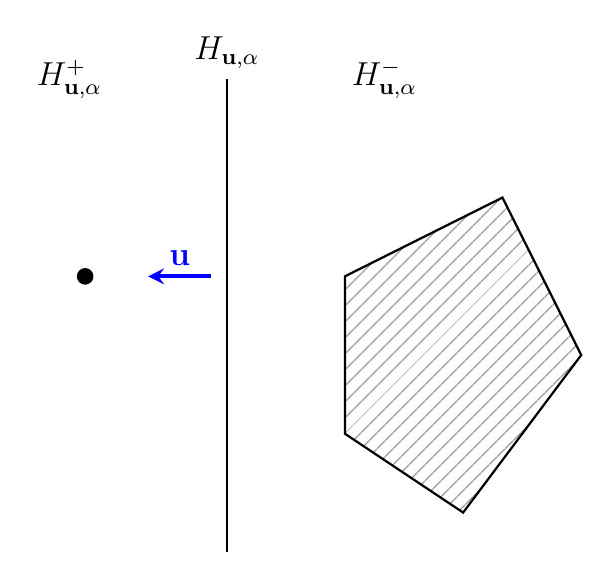
\begin{tikzpicture}
    \tikzset{
        every node/.style={font=\large},
        every path/.style={line width=1pt}
    }

    % 1. 定义关键坐标
    % 分离线的位置 x=0
    \coordinate (Top) at (0, 3);
    \coordinate (Bottom) at (0, -3);
    
    % 左侧的点
    \coordinate (PointLeft) at (-1.8, 0.5);
    
    % 右侧凸多边形的顶点 (五边形)
    \coordinate (P1) at (1.5, 0.5);  % 左上
    \coordinate (P2) at (3.5, 1.5);  % 右上
    \coordinate (P3) at (4.5, -0.5); % 右中
    \coordinate (P4) at (3.0, -2.5); % 右下
    \coordinate (P5) at (1.5, -1.5); % 左下

    % 2. 绘制分离平面 (Separating Hyperplane) H_{u, a}
    \draw (Bottom) -- (Top) node[above] {$H_{\mathbf{u}, \alpha}$};

    % 3. 绘制区域标注 (Half-spaces)
    % 左侧 H+
    \node at (-2, 3) {$H_{\mathbf{u}, \alpha}^+$};
    % 右侧 H-
    \node at (2, 3) {$H_{\mathbf{u}, \alpha}^-$};

    % 4. 绘制左侧的点
    \fill (PointLeft) circle (3pt);
    % 可选:如果需要标记点的名称,取消下面注释
    % \node[below left] at (PointLeft) {$x_0$};

    % 5. 绘制右侧凸体 (Convex Body)
    % 填充图案:白色斜线
    \fill[pattern={Lines[angle=45, distance=4pt, line width=0.5pt]}, pattern color=gray!80] 
        (P1) -- (P2) -- (P3) -- (P4) -- (P5) -- cycle;
    
    % 绘制轮廓
    \draw[thick] (P1) -- (P2) -- (P3) -- (P4) -- (P5) -- cycle;

    % 6. 绘制法向量 u (Normal Vector)
    % 蓝色,加粗,从分离线指向左侧
    \draw[->, >=stealth, color=blue, line width=1.5pt] 
        (-0.2, 0.5) -- (-1.0, 0.5) node[midway, above, text=blue] {$\mathbf{u}$};
        

\end{tikzpicture}

\end{document}